\documentclass{article}
\usepackage{iclr2027_conference,times}
\usepackage[utf8]{inputenc}
\usepackage[T1]{fontenc}
\usepackage{amsmath,amssymb,amsthm,bm}
\usepackage{booktabs}
\usepackage{multirow}
\usepackage{graphicx}
\usepackage{microtype}
\usepackage{xcolor}
\usepackage[colorlinks=true,linkcolor=blue,citecolor=blue,urlcolor=blue]{hyperref}

\newcommand{\E}{\mathbb{E}}
\newcommand{\pmm}[2]{#1{\scriptstyle\,\pm #2}}
\theoremstyle{plain}
\newtheorem{proposition}{Proposition}
\newtheorem{corollary}{Corollary}
\theoremstyle{definition}
\newtheorem{example}{Example}
\newcommand{\best}[1]{\bm{#1}}
\newcommand{\ours}[1]{#1\textsuperscript{\dag}}
\newcommand{\finding}[1]{\vspace{2pt}\noindent\textbf{Finding.}~~\emph{#1}\vspace{2pt}}

\title{Goal-Conditioned Q-Learning\\from Action-Free Data and Few Action Labels}

\author{Anonymous}

\begin{document}
\maketitle

\begin{abstract}
Offline goal-conditioned reinforcement learning assumes every transition carries an action label, yet the temporal structure of a control problem---which states lead to which---is visible in state-only experience, which is far more abundant. We study the regime where only a small fraction $p$ of trajectories retain actions, and ask what the labels must teach. Our answer is a factoring principle: \emph{action labels should only ever be asked to learn local, goal-free objects; every goal-dependent, long-horizon quantity can be learned action-free}. We instantiate the principle twice. \emph{Algebraically}, a bilinear value $V(s,g)=\varphi(s)^{\!\top}\psi(g)$ pulls the goal out of the expectation, so a one-step, goal-free expectation model $\mu(s,a)\!\approx\!\E[\varphi(s')|s,a]$ fit on labeled rows reconstructs $Q$ for every goal. \emph{Geometrically}, a quasimetric value pulls the goal out of the policy: labels train an actor only for near goals, and a closed-form geodesic waypoint over dataset states supplies long-horizon direction. On OGBench manipulation the algebraic form, with the expectation model written as a displacement rather than an absolute feature, matches at $p{=}0.10$ the action-conditioned learner trained on \emph{all} labels; on navigation the geometric form reaches $84.9$ at $p{=}0.10$, exceeding the full-label ceiling of its own substrate ($83.2$) without hierarchy or pseudo-labels. Controlled decompositions---crossed label oracles, label-corruption pricing, a direct goal-conditioned head as negative control, and grounding-slot swaps against imputation---show each half of the factoring is necessary, and locate exactly where labels still bind.
\end{abstract}

\section{Introduction}
Q-learning entangles two kinds of knowledge: \emph{temporal structure} (which states lead to which, and how far apart they are) and \emph{action grounding} (which action moves the agent along an edge). Only the second requires action labels. State-only experience---video, third-person demonstrations, logs missing actuation---carries the first in full. This asymmetry suggests a budgeted view of offline goal-conditioned RL (GCRL): given a dataset in which only a fraction $p$ of trajectories retain actions, what is the least the labels must teach?

The dominant answer is \emph{imputation}: fit an inverse dynamics model (IDM) on the labeled rows, pseudo-label every transition, and run a standard agent~\citep{ssorl}. Imputation is strong precisely when actions are identifiable from state pairs, but it answers the budget question indirectly---it converts the missing-label problem back into the fully-labeled one. We pursue the direct answer, and find it has a simple form:

\begin{quote}
\emph{Factor the goal out of everything the labels touch. Labels learn local, goal-free objects; all goal-dependence and long-horizon structure is learned action-free.}
\end{quote}

We call the resulting family \emph{action-free values} (AFV). A per-domain action-free \emph{substrate} is trained on all rows: an expectile-TD bilinear value for manipulation, a quasimetric value for navigation. Labels then ground control through one of two factorings. The \textbf{algebraic} factoring uses bilinearity to pull $\psi(g)$ out of the one-step expectation, $Q(s,a,g)=r+\gamma\,\E[\varphi(s')|s,a]^{\!\top}\psi(g)$, so labels fit only the goal-\emph{free} expectation model $\mu(s,a)$. The \textbf{geometric} factoring uses the triangle structure of a quasimetric to pull the goal out of the policy, $\pi(a\,|\,s,g)\rightarrow\pi(a\,|\,s,w(s,g))$: labels train an actor for goals at most $k$ steps away, and the waypoint $w$ is a closed-form argmin over dataset states---no hierarchy is learned. In both cases extraction is strictly in-sample (advantage-weighted regression); we show empirically that this is load-bearing, not a preference.

Our contributions: (i) the factoring principle and its two instantiations, one recipe with a per-domain substrate; (ii) a controlled evaluation against learner-matched imputation and leakage-audited action-conditioned baselines across manipulation and navigation at $p\in[0.02,0.5]$; (iii) an investigation that decomposes \emph{what labels buy} via crossed label oracles, label corruption, a direct goal-conditioned head as a negative control, and grounding-slot swaps. The investigation yields sharp answers: label cost is per-state \emph{actor coverage}, never model accuracy; the labels' entire value is the $s\!\to\!a$ correspondence; heads that must learn goal-dependence from labels fail, and fail faster as labels shrink; \emph{how} the goal-free model is parameterized is worth more than anything else inside the interface, and is a conditioning effect that pays at every budget rather than a label-efficiency one; and the geometric composition---not any particular grounding---is what conquers navigation, a result we establish by turning our own method's strongest control against it. An audit of the learned metric at scale closes the loop between theory and practice: the waypoint bound's assumptions name what fails on the large maze, and restoring them---a per-scale ring, short-range-only metric queries---turns a bimodal failure into the best number on the board.

\section{Preliminaries}
\label{sec:prelim}
We consider offline GCRL: a dataset $\mathcal{D}$ of trajectories in an MDP with states $s$, actions $a$, goals $g$ drawn from reached states, sparse reward $r(s,g)$, and discount $\gamma$. An agent trains offline and is evaluated on commanded goals. In the \emph{label-budget} setting a mask retains actions on a fraction $p$ of trajectories (labeled rows); all other rows are state-only $(s,s',g)$. We write $V(s,g)$ for a goal-conditioned value and $d(s,g)$ for a learned quasimetric (an asymmetric distance with $d(s,s)=0$ and triangle inequality, whose negation acts as a value)~\citep{qrl}.

\textbf{Substrates.} Both of our substrates train on \emph{every} row and read no actions (Figure~\ref{fig:substrate}). For manipulation we use an expectile-TD value~\citep{iql} in bilinear form $V(s,g)=\varphi(s)^{\!\top}\psi(g)/\sqrt{d}$ \citep{icvf}. For navigation we use QRL's quasimetric objective~\citep{qrl}. The substrate choice is dictated by the domain's temporal geometry (Section~\ref{sec:results}); no grounding strategy can exceed its substrate's full-label ceiling, so we report recovery relative to matched ceilings throughout.

\textbf{Baselines.} Semi-supervised offline RL (SS-ORL)~\citep{ssorl} imputes actions with an IDM fit on labeled rows; we always instantiate it with the \emph{same} substrate/learner as ours (SS-ORL-GCIVL on manipulation, SS-ORL-QRL on navigation), separating the imputation question from learner strength. Action-conditioned baselines (GCIQL) are leakage-audited: their value losses are masked to labeled rows, closing an inflation we measured at up to $20$ points at $p{=}0.05$.

\section{Method: two factorings of one principle}
\label{sec:method}
\textbf{Algebraic factoring (AFV-IVL, manipulation).}
With a bilinear substrate the one-step action-value is
\begin{equation}
Q(s,a,g) \;=\; r(s,g) + \gamma\,\E\!\left[V(s',g)\,\middle|\,s,a\right]
\;=\; r(s,g) + \gamma\,\underbrace{\E\!\left[\varphi(s')\,\middle|\,s,a\right]}_{\textstyle \mu(s,a)}{}^{\!\top}\,\psi(g)/\sqrt{d}.
\label{eq:factor}
\end{equation}
The goal leaves the expectation: the only object the labels must fit is the \emph{goal-free, one-step} expectation model $\mu(s,a)$, regressed on labeled rows onto $\varphi(s')$ in feature space; Proposition~\ref{prop:grounding} shows the errors that matter are the ones inside the span of goal embeddings, and the corresponding projected loss is reported as an ablation. A $K$-ensemble over $\mu$ provides pessimism via a lower-confidence bound on the disagreement. Policy extraction is behaviour-regularised deterministic policy improvement on the reconstructed $Q$ (DDPG${+}$BC). The improvement term at $a=\pi(s,g)$ requires no action label and is therefore \emph{definable} at every state, but we restrict it to labeled rows along with the cloning term: evaluating it everywhere collapses cube-single $p{=}0.10$ from $\pmm{67.8}{1.1}$ to $\pmm{5.7}{0.5}$ (one flag, three seeds each). The $K{=}5$ disagreement penalty does not prevent this --- $\mu$ is confidently wrong off the labeled states and the ensemble agrees with itself there --- so the policy is improved only where the labels reach.\  advantage-weighted regression (AWR)~\citep{awr} on the reconstructed $Q$ and reranking of dataset actions are reported as alternatives. Notably, the factorization buys mostly \emph{amortization} rather than accuracy: a monolithic head $q(s,g,a)$ regressed on the same frozen-value target reaches $\pmm{43.9}{6.7}$ at $p{=}0.10$ against the factored path's $\pmm{51.9}{5.1}$---an $8$-point gap whose bands overlap---but it must relearn goal-dependence from labels, which is what fails outright at low budgets (Section~\ref{sec:invest}).

\textbf{Geometric factoring (AFV-GEO, navigation).}
Navigation defeats the one-step form for a different reason: the binding constraint is not the model but the \emph{actor}, which sparse labels leave incompetent on most of the route (Section~\ref{sec:invest}). The quasimetric substrate supplies the fix, because its triangle structure factors long-horizon reaching through intermediate states: $d(s,g)\le d(s,w)+d(w,g)$, with near-equality along geodesics~\citep{horizongen}. We therefore (i) train the actor by AWR \emph{only on goals at most $k$ dataset steps ahead} ($k{=}25$)---the local job a small budget can cover---and (ii) at evaluation select, at every step, a waypoint from a bank $B$ of dataset states,
\begin{equation}
w^\ast(s,g)\;=\;\arg\min_{w\in B}\; \hat d(s,w)+\hat d(w,g)
\quad\text{s.t.}\quad \hat d(s,w)\in[0.5,1.5]\cdot \kappa,
\label{eq:waypoint}
\end{equation}
handing the actor $w^\ast$ instead of $g$ ($\kappa$ converts $k$ into learned-metric units, calibrated once per maze scale). One term of Eq.~\ref{eq:waypoint} asks the metric a question it cannot answer at scale: on the large maze $\hat d(w,g)$ spans distances where the learned metric saturates (Section~\ref{sec:invest}), so there we replace it by a graph cost-to-goal $c(w,g)$---the shortest-path cost from $w$ to $g$ over the bank, using as edges only pairs the metric can measure locally ($\hat d\le\rho$). The ``high level'' still has no parameters and is never trained; waypoints are dataset states and hence in-support by construction. Labels again learn a local, effectively goal-free object---the goal argument of the trained actor ranges only over a $k$-step ball. Proposition~\ref{prop:waypoint} bounds the cost of the composition.

\textbf{Extraction rule.} In both factorings the actor is trained by in-sample AWR and the critic is never evaluated at proposed actions. This is a hard constraint of the low-label regime: with DDPG+BC extraction the same geometric method collapses from $84.9$ to $0.2$.

\begin{figure}[t]
\centering
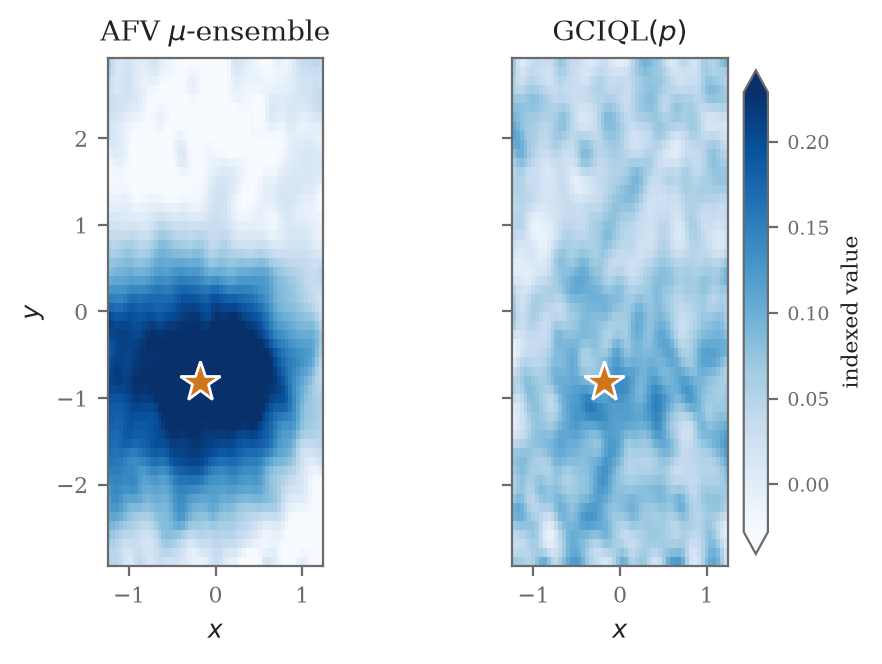
\includegraphics[height=1.62in]{figures/value_structure_cube.png}\hfill
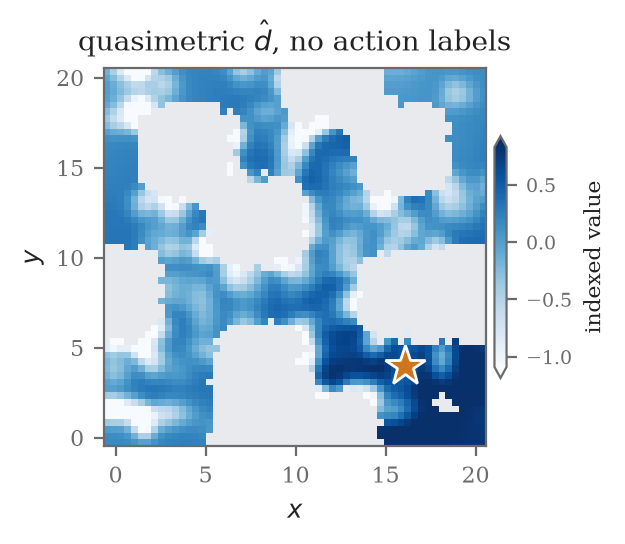
\includegraphics[height=1.62in]{figures/value_structure_antmaze.png}
\caption{\textbf{The structure the labels never touch.} Value fields over dataset states for a fixed goal (\textcolor{orange}{$\bigstar$}), indexed per method ($1$: one step from the goal; $0$: a random goal), count-weighted local averages; grey = no dataset support. \emph{Left pair} (cube-single, cube $(x,y)$, arm marginalized, $p{=}0.10$): the algebraic factoring's substrate---bilinear expectile $V$ trained on all rows without actions, grounded by $\mu$ on $10\%$ labels---forms a coherent field peaking at the goal, while the action-conditioned learner at the same budget does not. \emph{Right} (antmaze-medium): the geometric factoring's substrate---the quasimetric $\hat d$, trained with zero action labels---respects walls and grades along corridors; this is the field Eq.~\ref{eq:waypoint} plans through. Both fields exist before any label is spent on control.}
\label{fig:substrate}
\end{figure}

\section{Analysis: what each factoring guarantees}
\label{sec:theory}
Two propositions make the factoring principle precise; proofs are in Appendix~\ref{app:proofs}. Throughout, $\mathcal D$ is generated by a behavior policy, the label mask is drawn at the trajectory level independently of content, and on an unlabeled row the executed action is a latent variable with posterior $p(a\mid s,s')$. For any value $V$, write $Q_V(s,a,g):=r(s,g)+\gamma\,\E[V(s',g)\mid s,a]$ for its one-step lookahead (the middle term of Eq.~\ref{eq:factor}); if $V=V^\ast$ then $Q_V=Q^\ast$.

\textbf{Grounding bias.} The two grounding routes read a row differently: the algebraic factoring uses it only through $\varphi(s')$, whose conditional mean is the very object being estimated, while imputation writes a fabricated action into the row and treats it as real.

\begin{proposition}[Feature-mean grounding is exact; mean-action grounding is not]
\label{prop:grounding}
Let $V(s,g)=\varphi(s)^{\!\top}\psi(g)$ be any bilinear value (the $1/\sqrt d$ scale of Eq.~\ref{eq:factor} absorbed into $\psi$), let $\mu(s,a)=\E[\varphi(s')\mid s,a]$, $\Psi=\mathrm{span}\{\psi(g):g\in\mathcal G\}$, and $\Pi_\Psi$ the orthogonal projector onto $\Psi$.
\textbf{(i)} Under arbitrary dynamics, $r(s,g)+\gamma\,\mu(s,a)^{\!\top}\psi(g)=Q_V(s,a,g)$ for all $(s,a,g)$. For any estimate $\hat\mu$, the reconstruction $\hat Q:=r+\gamma\,\hat\mu^{\!\top}\psi(g)$ obeys
$|\hat Q(s,a,g)-Q_V(s,a,g)|\le\gamma\,\|\Pi_\Psi(\hat\mu(s,a)-\mu(s,a))\|_2\,\|\psi(g)\|_2$,
and on labeled rows $\varphi(s')$ is an unbiased regression target for $\mu(s,a)$---irrespective of the behavior policy and of any multi-modality of $p(a\mid s,s')$.
\textbf{(ii)} Assume deterministic dynamics $s'=f(s,a)$ and let $\hat a(s,s')=\E[a\mid s,s']$ be the imputed action (the Bayes-optimal inverse model under squared loss). Every pseudo-labeled row asserts the one-step constraint $Q(s,\hat a,g)=r(s,g)+\gamma V(s',g)$, whose bias against the true lookahead at $\hat a$ is
\begin{equation}
\gamma\,\big|V(s',g)-V(f(s,\hat a),g)\big|
\;=\;\gamma\,\Big|\E_{a\sim p(\cdot\mid s,s')}\big[V(f(s,a),g)\big]-V\big(f(s,\E[a\mid s,s']),g\big)\Big|,
\label{eq:jensen}
\end{equation}
a Jensen gap of $a\mapsto V(f(s,a),g)$ across the posterior. It is zero if and only if $\hat a(s,s')$ is value-equivalent to the posterior's support---in particular whenever the posterior is a point mass---and Example~\ref{ex:modes} makes it $\gamma^2/(1-\gamma)$---of order the value range---on four states.
\end{proposition}

\begin{corollary}[Identifiability governs the contest]
\label{cor:ident}
If actions are identifiable from state pairs ($p(a\mid s,s')$ a point mass a.e.), the bias \eqref{eq:jensen} vanishes identically: on such data the two groundings differ only in estimation error. Conversely, any corruption that spreads $p(a\mid s,s')$ across actions not value-equivalent to their mean injects the bias into imputation only, while the regression target in (i) remains unbiased; observation noise is such a corruption, whereas behavior-policy noise under injective dynamics is not.
\end{corollary}

Three readings. \emph{First}, on cube, state pairs determine ${\sim}96\%$ of action variance, so Corollary~\ref{cor:ident} predicts the observed draw with matched SS-ORL---and says no experiment on this data can separate the groundings; our claims do not rest on beating imputation there. \emph{Second}, the estimation clause of (i) is why the label-side problem is small: $\mu$ is goal-free, fit once for every goal from all $p\!\cdot\!N$ labeled rows, with only its $\Psi$-projection visible; a direct head $q(s,g,a)$ enjoys none of this and must relearn the goal-half of $Q$ from the same rows---Section~\ref{sec:invest} prices the difference ($36.7$ vs $51.9$ at $p{=}0.10$, widening at $p{=}0.05$). \emph{Third}, Example~\ref{ex:modes} exposes an asymmetry in-sample extraction cannot repair: imputation \emph{fabricates} the dataset actions it then treats as in-sample, so restricting to dataset actions protects AFV (whose labeled actions are real) but not imputation. The converse clause of Corollary~\ref{cor:ident} is falsifiable: as observation noise grows, imputation acquires a bias feature-mean grounding does not; both degrade through $V$ itself, so the prediction is \emph{differential} degradation. We pre-registered and ran this sweep; the outcome (Section~\ref{sec:invest}) is negative in an instructive way.

\textbf{Waypoint composition.} The geometric factoring composes three objects: a quasimetric $\hat d$ trained on all rows, a bank $B$ of dataset states, and an actor trained only on near goals. The guarantee is a per-segment overhead bound; the horizon multiplies only quantities that cost no labels.

\begin{proposition}[Per-segment suboptimality of the waypoint policy]
\label{prop:waypoint}
Consider deterministic goal-reaching, $d^\ast(x,y)$ the minimal number of steps from $x$ to $y$, and the policy of Eq.~\ref{eq:waypoint} with ring $[k_-,k_+]$: command $g$ if $\hat d(s,g)\le k_+$, else the waypoint $w^\ast(s,g)$, held until reached. Assume
\textbf{(i)} \emph{metric accuracy:} $|\hat d(x,y)-d^\ast(x,y)|\le\varepsilon$ for every pair the planner can query, $(x,y)\in\mathcal S\times(B\cup\{g\})$;
\textbf{(ii)} \emph{bank coverage with slack $\delta$:} every $s$ with $d^\ast(s,g)>k_+-\varepsilon$ admits $w\in B$ with $d^\ast(s,w)\in[k_-+\varepsilon,\,k_+-\varepsilon]$ and $d^\ast(s,w)+d^\ast(w,g)\le d^\ast(s,g)+\delta$;
\textbf{(iii)} \emph{band competence with overhead $\alpha$:} commanded any $w\in B\cup\{g\}$ with $d^\ast(s,w)\le k_++\varepsilon$, the actor reaches $w$ within $d^\ast(s,w)+\alpha$ steps.
If $k_->5\varepsilon+\delta$, then from every $s_0$ the waypoint policy reaches $g$ in at most
\begin{equation}
T\;\le\;d^\ast(s_0,g)\;+\;N\,(\alpha+\delta+4\varepsilon)\;+\;\alpha,
\qquad
N\;\le\;\Big\lceil\tfrac{d^\ast(s_0,g)}{k_--5\varepsilon-\delta}\Big\rceil ,
\label{eq:wpbound}
\end{equation}
steps: the optimal cost plus a fixed overhead per segment, the horizon entering only through the segment count $N$.
\end{proposition}

With $\varepsilon=\delta=\alpha=0$ the bound collapses to optimality and recovers planning invariance---the optimal policy's indifference between $g$ and a geodesic waypoint~\citep{horizongen}; Proposition~\ref{prop:waypoint} is the quantitative version for a learned metric and a finite bank, in the lineage of search over replay buffers~\citep{sorb}.

\begin{corollary}[Labels must cover the band, not the horizon]
\label{cor:band}
In Proposition~\ref{prop:waypoint}, action labels enter only through $\alpha$, a property of the actor on the band $\{(s,w):d^\ast(s,w)\le k_++\varepsilon\}$; $\varepsilon$ and $\delta$ belong to objects built without labels ($\hat d$ from all rows, $B$ a subsample of dataset states). The demand on labeled data is coverage of the band, which does not grow with the commanded horizon, and the supply is dense: a labeled trajectory of length $L$ contains at least $(L-k_+)\,k_+$ in-band state--goal pairs. (This locates which pairs labels must cover; it is not a finite-sample bound, and we impose no generalization assumptions on the actor.)
\end{corollary}

This is the label-efficiency asymmetry of Section~\ref{sec:invest} stated ex ante: a flat actor's problem grows with the task horizon and its curve in $p$ is steep ($29.0\rightarrow56.9\rightarrow81.5$), while the composed actor's problem does not grow, and $p{=}0.10$ is already dense for it ($84.9$). Two honest notes. The bound does not cap the method at the flat learner's full-label ceiling---the composed policy class is different, which is how $84.9$ can exceed $83.2$ without contradiction---and it does not by itself explain that excess. And its assumptions localize the observed failure at scale: (i) holds for our learned $\hat d$ only at short range---the metric compresses long distances---so on antmaze-large the one-hop score $\hat d(w,g)$ ranked far waypoints noisily and the medium-calibrated ring selected waypoints outside the useful band. Section~\ref{sec:invest} measures this and repairs it inside the bound's own vocabulary: restore (i) by querying $\hat d$ only at short range (the graph cost-to-goal), restore (ii) by recalibrating the ring per scale. The deployed planner also idealizes the proposition in two places (reach threshold and hysteresis in place of exact arrival and hold-until-arrival; Appendix~\ref{app:proofs}).

\section{Results}
\label{sec:results}
\begin{table}[t]
\centering
\caption{Success rate ($\times 100$, mean of final three evaluations, $n{=}3$ seeds; $\pm$ is std over seeds) across OGBench domains and label budgets $p$. \dag: composition introduced in this paper (both groundings). SS-ORL is learner-matched per domain. GCIQL is leakage-audited. HIQL$(p)$ (high level action-free, low level labeled) is reported as evidence for the decomposition, not as a member of our flat method class. Full = all labels. GEO rows use the planner calibrated per maze scale (ring + graph cost-to-goal on large; Section~\ref{sec:invest}); $\ddagger$: cell predates the planner recalibration and is being re-scored. $\S$: pooled over $3$ label draws $\times\,3$ seeds ($n{=}9$); all other cells are one label draw, whose error bars therefore omit a draw term we measure to be comparable to the seed term (Section~\ref{sec:invest}). Full-label cube ceilings are our own matched-protocol runs, reproduced with $n{=}3$ rather than quoted.}
\label{tab:main}
\vspace{2pt}
\small
\setlength{\tabcolsep}{3.2pt}
\begin{tabular}{l cccc c}
\toprule
\multicolumn{6}{c}{\emph{Manipulation (cube-single; cube-double at $p{=}0.10$, 1M steps)}}\\
\cmidrule(lr){1-6}
 & $p{=}.02$ & $p{=}.05$ & $p{=}.10$ & $p{=}.20$ & double \\
\midrule
AFV-IVL, direct $\mu$ & $\pmm{22.9}{3.0}$ & $\pmm{44.2}{2.6}$ & $\pmm{51.9}{5.1}$ & $\pmm{51.6}{5.3}$ & $\pmm{4.8}{1.2}$ \\
AFV-IVL, residual $\mu$ (ours) & $\pmm{26.8}{2.7}$ & $\best{\pmm{60.3}{3.6}}$\rlap{$^{\S}$} & $\best{\pmm{72.4}{5.9}}$\rlap{$^{\S}$} & --- & --- \\
SS-ORL (matched) & $\best{\pmm{48.5}{4.2}}$ & $\pmm{50.9}{3.8}$ & $\pmm{50.7}{8.6}$ & $\pmm{53.3}{1.8}$ & $\best{\pmm{30.6}{2.8}}$ \\
GCIQL (audited) & $\pmm{10.0}{2.2}$ & $\pmm{39.3}{4.5}$ & $\pmm{66.9}{7.5}$ & $\pmm{55.8}{11.7}$ & $\pmm{0.8}{0.2}$ \\
\midrule
substrate ceiling (full) & \multicolumn{4}{c}{GCIVL $\pmm{56.4}{5.6}$ \qquad GCIQL $\pmm{70.6}{3.7}$} & $36$ \\
\midrule
\multicolumn{6}{c}{\emph{Navigation (antmaze-medium / antmaze-large)}}\\
\cmidrule(lr){1-6}
 & \multicolumn{2}{c}{med $p{=}.02$ / $.05$} & med $p{=}.10$ & large $p{=}.05$ & large $p{=}.10$ \\
\midrule
AFV-QRL (no comp.) & \multicolumn{2}{c}{--- / ---} & $\pmm{29.0}{1.3}$ & --- & $\pmm{2.4}{0.5}$ \\
AFV-GEO\textsuperscript{\dag} (ours) & \multicolumn{2}{c}{$\pmm{59.1}{3.1}$ / $\pmm{72.9}{2.8}$} & $\best{\pmm{84.9}{3.0}}$ & $\pmm{7.2}{6.4}^{\ddagger}$ & $\pmm{52.4}{8.6}$ \\
SS-ORL-QRL (matched) & \multicolumn{2}{c}{$\pmm{68.9}{3.7}$ / $\pmm{70.6}{14.1}$} & $\pmm{71.7}{15.1}$ & $\best{\pmm{68.4}{5.8}}$ & $\pmm{71.4}{3.1}$ \\
SS-ORL-GEO\textsuperscript{\dag} (control) & \multicolumn{2}{c}{$\best{\pmm{92.9}{2.0}}$ / $\best{\pmm{93.1}{2.7}}$} & $\pmm{83.5}{10.4}$ & --- & $\best{\pmm{92.5}{0.5}}$ \\
HIQL$(p)$ (evidence) & \multicolumn{2}{c}{$\pmm{77.6}{1.4}$ / $\pmm{87.6}{1.5}$} & $\pmm{91.7}{1.6}$ & $\pmm{68.1}{7.3}$ & $\pmm{74.7}{1.5}$ \\
\midrule
substrate ceiling (full QRL) & \multicolumn{2}{c}{$83.2$} & $83.2$ & $76.3$ & $76.3$ \\
\bottomrule
\end{tabular}
\end{table}

We evaluate on OGBench~\citep{ogbench} manipulation (cube-single, cube-double) and navigation (antmaze-medium/large, navigate datasets), $p\in\{0.02,0.05,0.10,0.20,0.50\}$, three seeds, protocol fixed before each wave (bars pre-registered in launch scripts). Table~\ref{tab:main} is the cross-domain picture; three readings matter.

\textbf{Manipulation: how the grounding model is parameterized decides the domain.} Written directly, $\mu$ regresses onto $\phi(s')$; written as a displacement, $\mu(s,a)=\phi(s)+\Delta(s,a)$, the labels no longer pay to re-derive $\phi(s)$---which the substrate already supplies exactly from unlabeled data---and $\Delta{=}0$ becomes the prior ``this action changes nothing''. $\Delta$ keeps the signature $(s,a)$, so it stays goal-free and the amortization of Eq.~\ref{eq:factor} is untouched. The change is worth $+16.1$ at $p{=}0.05$ and $+20.5$ at $p{=}0.10$ (pooled over three label draws), and it moves the cube verdict: the direct form loses to matched imputation at every budget, while the residual form beats it by $+9.4$ at $p{=}0.05$ and $+21.7$ at $p{=}0.10$ with disjoint bands. At $p{=}0.10$ the residual reaches $\pmm{72.4}{5.9}$ against a reproduced full-label GCIQL oracle of $\pmm{70.6}{3.7}$: from a tenth of the actions it \emph{matches} the action-conditioned learner trained on all of them (the bands overlap; we claim parity, not excess). At $p{=}0.02$ imputation still wins ($48.5$ vs $26.8$), and that is the honest boundary---on cube, state pairs determine ${\sim}96\%$ of action variance, so an IDM fit on $2\%$ of trajectories already imputes near-perfectly, and no grounding-side change can beat a near-exact one at budgets that small. Cube-double is the open failure: imputation wins decisively ($30.6$ vs $4.8$), and diagnosing it is ongoing work.

\textbf{Navigation: the geometric factoring is the discovery.} The one-step form transplants poorly ($29.0$ at $p{=}0.10$ with the matched substrate), and no amount of budget rescues it below $p{\approx}0.5$ (Section~\ref{sec:invest}). AFV-GEO reaches $\pmm{84.9}{3.0}$---above its substrate's \emph{full-label} ceiling ($83.2$), above matched imputation ($71.7$), with no hierarchy and no pseudo-labels. On antmaze-large the recipe first collapsed for \emph{both} groundings with severe seed variance---which is what told us the failure was in the shared planner, not the labels. Section~\ref{sec:invest} traces it to long-range saturation of the learned metric and repairs it with a per-scale ring and a graph cost-to-goal over the bank. Under the repaired planner the composition itself is strong at scale (${\sim}91$ when grounded with full labels or imputed actions, above the flat full-label ceiling of $76.3$), and AFV-GEO reaches $\pmm{52.4}{8.6}$ from a dead $2.4$: what binds on large is no longer the mechanism but label coverage of the actor's band.

\textbf{The composition, not the grounding, wins navigation.} Applying the full geometric recipe on top of \emph{imputed} actions (SS-ORL-GEO---a method that does not exist in prior work; we introduce it as a control) matches AFV-GEO at medium $p{=}0.10$ ($83.5$ vs $84.9$) and dominates everywhere else it has been run: $92.9$ at medium $p{=}0.02$ and $\pmm{92.5}{0.5}$ on large $p{=}0.10$, both above the flat full-label ceilings. The factoring principle is the transferable content; the grounding slot is swappable. What AFV's label-side grounding adds over imputation is architectural---one fewer trained model, no pseudo-label bias, $3\times$ lower seed variance at parity---but the parity itself holds only where the labeled trajectories densely cover the actor's band (medium at $p{=}0.10$); everywhere the coverage thins (medium $p{\le}0.05$, large at every tested $p$), imputation-grounding currently wins the slot.

\section{Investigation: what do the labels actually buy?}
\label{sec:invest}
\textbf{Label cost is actor coverage, not model accuracy.} Crossed oracles at antmaze-medium $p{=}0.10$: granting the \emph{actor} all labels (value and dynamics stay masked) lifts $29.0\rightarrow\pmm{86.3}{2.6}$; granting the \emph{dynamics model} all labels yields $\pmm{35.3}{2.4}$. The entire $57$-point gap is per-state actor coverage. On cube the same oracles buy ${+}0.1$ and ${-}5.6$---both components are label-saturated at $p{=}0.10$. This is the empirical basis for the factoring: the only thing labels must buy is local competence, so the method should never ask them for more. It also bounds what any grounding-side change can be worth on navigation: the dynamics oracle caps that component at ${+}6.3$, so an improvement there is not where a large antmaze gain could come from, and we do not claim one.

\textbf{The residual parameterization is a conditioning effect, not a label-efficiency one.} It is tempting to read the cube result as ``labels go further''---the bar it passed was a low-budget bar---but the measured shape says the opposite: the gain over the direct form is $+3.9$, $+16.1$, $+20.5$ at $p{=}0.02,0.05,0.10$, i.e.\ \emph{smallest} where labels are scarcest. Two independent facts with opposite budget-shapes must not be conflated. Having a grounding model at all is the scarce-label story: against an in-sample AWR floor that builds no model, $\mu$-grounding is worth $+15.8$ and $+17.0$ at $p{=}0.02,0.05$ and $-1.3$ at $p{=}0.10$, where it is redundant. How that model is \emph{parameterized} is a conditioning story that pays at every budget. Navigation confirms the second half on a different substrate: QRL's latent dynamics model has always been residual-structured, and ablating that structure costs $83.2\rightarrow\pmm{62.4}{11.3}$ at full labels and $29.0\rightarrow\pmm{12.8}{3.5}$ at $p{=}0.10$---load-bearing at both budgets. Transplanting the residual onto a substrate whose \emph{value} is weak buys nothing ($\pmm{2.8}{1.1}$ vs $\pmm{2.8}{1.3}$ on the flat GCIVL learner at antmaze-medium): a grounding-side change cannot repair a substrate-side failure, which is the decomposition of Section~\ref{sec:results} appearing as a null result.

\textbf{Which trajectories are labeled matters as much as which seed is trained.} Repeating the residual cells over three independent label draws, the draw-to-draw std is $3.4$ at $p{=}0.05$ and $4.5$ at $p{=}0.10$, against seed-to-seed stds of $2.5$ and $5.0$. The shape above survives ($+16.1<+20.5$ pooled, both clear of zero, neither cell's draw-std as large as half its gain), but the single-draw cells that fill the rest of Table~\ref{tab:main}---for every method, ours and baselines alike---carry an unmeasured term of this size. We flag it rather than repair it: pooling draws everywhere would multiply the compute of every cell in the paper.

\textbf{Two domains price labels oppositely.} Cube's dose curve is flat at ceiling from $p{=}0.10$; antmaze-medium's is steep ($29.0\rightarrow 56.9\rightarrow 81.5$ at $p{=}0.1,0.2,0.5$) until the composition removes the global demand on the actor, after which $p{=}0.10$ exceeds the full-label ceiling. ``How many labels are needed'' is not a well-posed benchmark question without stating which regime the domain is in.

\textbf{Labels are worth exactly their $s\!\to\!a$ correspondence.} Corrupting labeled actions on cube while keeping all states and masks byte-identical---shuffling real actions among labeled rows, or replacing them with a random policy's---sends AFV from $51.9$ to $0.0$ in both cases. The action-distribution prior is worth nothing; the correspondence is everything; and no unlabeled pathway leaks supervision.

\textbf{Learning goal-dependence from labels is the failure mode.} As a negative control we fit a direct head $q(s,g,a)$ on labeled rows toward the frozen target $r+\gamma V(s',g)$ and extract by AWR on $q-V$. It is worse than the factored path everywhere and degrades fastest as labels shrink ($36.7$ vs $51.9$ at $p{=}0.10$; $16.2$ vs $44.2$ at $p{=}0.05$): the head must relearn the goal-half of $Q$ from $p\cdot N$ samples, precisely the half the substrate provides for free in Eq.~\ref{eq:factor}. Meanwhile the corrected monolithic-$Q$ control reaches $\pmm{43.9}{6.7}$ against $\pmm{51.9}{5.1}$ at a matched budget: an $8$-point gap that we do not claim, since the bands overlap. Its contribution is amortizing goal-dependence, not representational power. (An earlier version of this control reported a $45$-point gap; that cell was invalidated by a broadcasting bug, and a mid-training read of the repaired run then suggested parity. $\pmm{43.9}{6.7}$ is the converged $n{=}3$ number.)

\textbf{Attribution of the navigation win.} Three controls pin the composition's mechanism. Eval-time waypoints on a stock-trained actor rescue nothing ($29.0\rightarrow 28.3$): near-goal \emph{training} is essential. Eval-time waypoints on stock imputation rescue nothing ($71.7\rightarrow 69.9$): a globally-trained actor has nothing to shrink. Replacing AWR with DDPG+BC collapses the method ($0.2$): in-sample extraction is load-bearing. Behaviorally, the pre-composition failure is sharp---the AFV-QRL antmaze policy moves $0.10$ units in its final $100$ steps (it freezes; it does not navigate badly) while its value ranks states correctly, exactly the signature of structure without local grounding.

\textbf{What breaks at scale: the learned metric is only locally accurate.} On antmaze-large the composition initially collapsed for \emph{both} groundings (means in the $30$s--$40$s, seed spreads above $20$)---a shared failure, so we audited the shared component. Probing $\hat d$ against ground-truth shortest paths (breadth-first search on the dataset's occupancy map) shows the metric tracks true distance up to ${\sim}150$ steps and then saturates: pairs $200$ and $500$ true steps apart differ by under a third in $\hat d$. The one-hop objective of Eq.~\ref{eq:waypoint} queries exactly that regime---$\hat d(w,g)$ spans most of the maze---so on large the argmin ranked far waypoints close to randomly: the chosen waypoint advanced the agent a median of $7$ true steps and pointed \emph{backward} on $24\%$ of selections. Medium tolerates the same per-selection noise because its tasks are short ($\le 181$ steps); large's $344$-step tasks exhaust the episode budget, and whether a seed clears them becomes a coin flip---the observed bimodality. Two changes repair it, each restoring an assumption of Proposition~\ref{prop:waypoint} where it measurably failed: recalibrating the ring per maze scale so selected waypoints land inside the actor's competence band (median forward progress doubles; backward selections drop to $15\%$), and replacing the saturated long-range term $\hat d(w,g)$ by the graph cost-to-goal of Section~\ref{sec:method}, which needs $\hat d$ only at short range. With both, the imputation-grounded control jumps from unstable ${\sim}40$ to $\pmm{92.5}{0.5}$ and the full-label composition from $38.0$ to $\pmm{90.9}{0.6}$---above the flat full-label ceiling of $76.3$---while medium is unchanged ($85.0$ vs $84.9$). Bank size and ring emptiness are ruled out (doubling the bank three times changes nothing; the feasible ring was never empty). What the repair exposes is a label-side gap: under the same planner the $10\%$-label near-goal actor reaches $\pmm{52.4}{8.6}$ while full labels or imputed actions reach ${\sim}91$. Our reading, not yet isolated experimentally: the large maze spreads the same number of labeled trajectories over more states, so per-state coverage of the actor's band---the one quantity Corollary~\ref{cor:band} says labels must supply---thins below what near-goal training needs.

\textbf{The observation-noise test of the premise comes back negative (for now).} Corollary~\ref{cor:ident} predicts observation noise should hurt imputation-grounding more than feature-mean grounding. We pre-registered and ran the sweep on cube-single at $p{=}0.05$: Gaussian noise of $\sigma\in\{0.1,0.3,1.0\}$ per-dimension standard deviations added to every stored observation (the log stays self-consistent; the evaluation environment is clean), which raises the fraction of action variance the state pair fails to explain from $0.04$ to $0.12$, $0.22$, $0.50$. The result is a floor, not a crossover: AFV falls $44.2\rightarrow 0.0$ already at $\sigma{=}0.1$ and never learns; matched SS-ORL falls $50.9\rightarrow 5.6$; both sit at $0.0$ from $\sigma{=}0.3$. At these levels the corruption destroys the shared substrate---$V$ itself---before any grounding-bias difference can express itself, and taken at face value the pre-registered prediction fails: the feature-mean arm degraded no slower than imputation. We report this as a negative result with one caveat: AFV's collapse is total from the first evaluation---a cliff, not a dose-response---and we have not yet isolated why. Either way, the differential-degradation prediction currently has no empirical support at any tested $\sigma$.

\section{Related work}
Semi-supervised offline RL imputes missing actions with an IDM~\citep{ssorl}; unlabeled-data methods reweight or share data across tasks~\citep{uds,pds}. Latent-action models learn pseudo-actions from video~\citep{lapo,lamlearn}. Action-free pretraining learns values or representations from state-only data~\citep{icvf,vip,hilp}; QRL learns quasimetric values~\citep{qrl}; HIQL extracts a two-level policy from one value~\citep{hiql} and is the hierarchical relative of our closed-form composition. Waypoint search over a learned distance traces to SoRB~\citep{sorb}; planning invariance~\citep{horizongen} is the exact-metric limit of Proposition~\ref{prop:waypoint}. Expectation models for values trace to \citet{wan2019expectation}; our $\mu$ is their goal-factored, label-budgeted instance. Our setting differs from all of the above in asking \emph{which information} labels must carry, and answering with a factoring principle evaluated under matched substrates and audited baselines.

\section{Discussion and limitations}
A single principle---factor the goal out of everything labels touch---covers both of our domains, but its instantiations are substrate-typed: algebraic where tasks are short-horizon funnels, geometric where they are metric routes. The typing is not a stylistic choice: transplanting the geometric factoring onto manipulation (quasimetric substrate plus near-goal actor and waypoints, \emph{full} labels, two calibrated near-goal bands) reaches only $2.4$ on cube-single against the expectile substrate's $54.9$---the metric, not the extraction, is what fails there, so the per-domain substrate is load-bearing. Open problems: the label side of antmaze-large, where the repaired planner exposes a band-coverage gap ($52.4$ for the $10\%$-label actor against ${\sim}91$ for its full-label and imputed counterparts); cube-double, where imputation currently wins and the composition has no metric substrate to ride; and the identifiability frontier---on state-based benchmarks actions are largely recoverable from state pairs, so imputation is near-free supervision, and our first attempt to move the frontier with observation noise collapsed both methods before it could discriminate (Section~\ref{sec:invest}). Constructing data that weakens action identifiability without destroying value learning itself---visual observations with aliasing are the natural candidate---is, on our evidence, the open experimental problem of the label-budget setting.

\bibliography{references}
\bibliographystyle{iclr2027_conference}

\appendix
\section{Proofs}
\label{app:proofs}

\subsection{Proof of Proposition~\ref{prop:grounding}}
\textbf{(i)} $\psi(g)$ is constant in $s'$, so by linearity of expectation
$\E[\varphi(s')^{\!\top}\psi(g)\mid s,a]=\E[\varphi(s')\mid s,a]^{\!\top}\psi(g)=\mu(s,a)^{\!\top}\psi(g)$,
which is the identity; no property of the dynamics is used. For the error bound, $\psi(g)\in\Psi$ gives
$(\hat\mu-\mu)^{\!\top}\psi(g)=\big(\Pi_\Psi(\hat\mu-\mu)\big)^{\!\top}\psi(g)$, and Cauchy--Schwarz finishes.
For unbiasedness: the mask is drawn at the trajectory level independently of content, so a labeled row is distributed as a dataset row; on it, $s'\sim P(\cdot\mid s,a)$ by definition of the generative process, hence $\E[\varphi(s')\mid s,a]=\mu(s,a)$. Multi-modality of $p(a\mid s,s')$ is a statement about the \emph{reverse} conditional and never enters the forward conditional mean.

\textbf{(ii)} Fix a dataset transition $(s,s')$ and let $a$ be its latent action, $a\sim p(\cdot\mid s,s')$. Under deterministic dynamics, every $a$ in the support satisfies $f(s,a)=s'$, so $V(f(s,a),g)=V(s',g)$ for all supported $a$, and therefore
$\E_{a\sim p(\cdot\mid s,s')}[V(f(s,a),g)]=V(s',g)$.
The pseudo-labeled row trains the pair $\big(\hat a(s,s'),\,r(s,g)+\gamma V(s',g)\big)$, i.e.\ asserts $Q(s,\hat a,g)=r(s,g)+\gamma V(s',g)$, while the true one-step lookahead at $\hat a$ is $Q_V(s,\hat a,g)=r(s,g)+\gamma V(f(s,\hat a),g)$. Subtracting gives \eqref{eq:jensen}. The gap is zero for all $g$ iff $V(f(s,\hat a),\cdot)=V(s',\cdot)$, i.e.\ iff $\hat a$ is value-equivalent to the posterior's support. If the posterior is a point mass, $\hat a$ equals the executed action, $f(s,\hat a)=s'$, and the gap vanishes. \hfill$\square$

We analyze the bias each pseudo-labeled row injects; how it propagates depends on the downstream learner, and a trained inverse model adds estimation error on top of the Bayes-optimal $\hat a$ analyzed here.

\subsection{Proof of Corollary~\ref{cor:ident}}
The first clause is the point-mass case of (ii). For the second: under deterministic, fully observed dynamics with $f(s,\cdot)$ injective, $a$ is a measurable function of $(s,s')$ and the posterior is a point mass \emph{regardless of the behavior policy}---behavior noise widens the marginal over actions, not the conditional given the transition. Only degeneracy of $f(s,\cdot)$ (Example~\ref{ex:modes}) or corruption of the observed pair can spread the posterior. For observation noise, let $o=h(s)+\eta$ be the observed process and let $V,\varphi,\hat a$ operate on observations, as they must. The identity in (i) is unaffected: $\mu(o,a)=\E[\varphi(o')\mid o,a]$ is by definition the conditional mean under the observed process, and $\varphi(o')$ on a labeled row remains an unbiased sample of it. For imputation, the pseudo-row $(o,\hat a(o,o'),o')$ asserts $Q(o,\hat a,g)=r+\gamma V(o',g)$ while the lookahead at $\hat a$ is $r+\gamma\,u(\hat a)$ with $u(a):=\E[V(o',g)\mid o,a]$; the per-row gap $\gamma|V(o',g)-u(\hat a)|$ no longer vanishes at the posterior's modes once $h$ (or $\eta$) aliases states, and its row-average over transitions sharing $(o,o')$ is the same Jensen structure with $u$ in place of $V(f(s,\cdot),g)$. \hfill$\square$

\subsection{The two-mode construction}
\begin{example}[A mean of modes is an action no mode takes]
\label{ex:modes}
States $\{s_0,s_1,s_w,g\}$, actions $\mathcal A=[-1,1]$, deterministic dynamics: $f(s_0,a)=s_1$ if $|a|\ge\tfrac12$ and $f(s_0,a)=s_w$ otherwise; $f(s_1,a)=g$ and $f(s_w,a)=s_w$ for all $a$. Rewards follow the goal-reaching convention ($-1$ per step until $g$, termination at $g$), so $V^\ast(s_1,g)=-1$, $V^\ast(s_w,g)=-\tfrac1{1-\gamma}$, $V^\ast(s_0,g)=-1-\gamma$. The behavior policy at $s_0$ plays $a=\pm\tfrac34$ with probability $\tfrac12$ each; every observed transition from $s_0$ lands in $s_1$, so the posterior is $p(a\mid s_0,s_1)=\tfrac12\delta_{-3/4}+\tfrac12\delta_{+3/4}$ and the Bayes-optimal imputation is $\hat a=\E[a\mid s_0,s_1]=0$---an action neither mode takes, and one that enters the trap: $f(s_0,0)=s_w$.

\emph{Imputation.} Every unlabeled $s_0$-row becomes $(s_0,\,0,\,s_1)$ and asserts $Q(s_0,0,g)=-1+\gamma V^\ast(s_1,g)=-1-\gamma$, while $Q^\ast(s_0,0,g)=-1+\gamma V^\ast(s_w,g)=-1-\tfrac{\gamma}{1-\gamma}$: the bias \eqref{eq:jensen} equals $\gamma\big(\tfrac1{1-\gamma}-1\big)=\tfrac{\gamma^2}{1-\gamma}$, of order the value range and diverging as $\gamma\to1$. Worse, the fabricated action dominates the pseudo-labeled dataset (a fraction $1-p$ of $s_0$-rows), so behavior-regularized extraction---BC, AWR, or any in-sample scheme, which all trust dataset actions---is pulled toward $a=0$ and the trap; ``in-sample'' offers no protection when the samples themselves are fabricated.

\emph{Feature-mean grounding.} Take $d=4$, $\varphi$ the one-hot state indicator, and $\psi(g)$ the vector of optimal values, so $V=V^\ast$ is bilinear-realizable. On the labeled rows the regression target for $\mu(s_0,\pm\tfrac34)$ is $\varphi(s_1)$, which is exact, and Proposition~\ref{prop:grounding}(i) reconstructs $Q^\ast$ at every labeled action; in-sample extraction weighs only the real actions $\pm\tfrac34$, both optimal, and never queries $\mu$ at the fabricated $a=0$. On identical rows, one grounding is exact and the other misses by the value range.
\end{example}

\subsection{Proof of Proposition~\ref{prop:waypoint}}
Call a step of the outer loop a \emph{segment}: the planner selects a command (either $g$ or a waypoint), and the actor runs until the command is reached. Write $s_i$ for the state starting segment $i$, $s_0$ the initial state, and $\Delta:=k_--5\varepsilon-\delta>0$.

\emph{Near case.} If $\hat d(s_i,g)\le k_+$, then by (i) $d^\ast(s_i,g)\le k_++\varepsilon$, (iii) applies with $w=g$, and the actor reaches $g$ within $d^\ast(s_i,g)+\alpha$ steps, ending the episode.

\emph{Far case.} If $\hat d(s_i,g)>k_+$, then by (i) $d^\ast(s_i,g)>k_+-\varepsilon$, so (ii) supplies a candidate $w^0\in B$ with $d^\ast(s_i,w^0)\in[k_-+\varepsilon,k_+-\varepsilon]$, hence $\hat d(s_i,w^0)\in[k_-,k_+]$: the feasible ring is nonempty and contains $w^0$. The selected $w_i=w^\ast(s_i,g)$ then satisfies
\[
\hat d(s_i,w_i)+\hat d(w_i,g)\;\le\;\hat d(s_i,w^0)+\hat d(w^0,g)\;\le\;d^\ast(s_i,w^0)+d^\ast(w^0,g)+2\varepsilon\;\le\;d^\ast(s_i,g)+\delta+2\varepsilon,
\]
and applying (i) once more to the left side,
\begin{equation}
d^\ast(s_i,w_i)+d^\ast(w_i,g)\;\le\;d^\ast(s_i,g)+\delta+4\varepsilon.
\label{eq:segment}
\end{equation}
Feasibility gives $d^\ast(s_i,w_i)\in[k_--\varepsilon,\,k_++\varepsilon]$, so (iii) applies: the actor reaches $w_i$ within $d^\ast(s_i,w_i)+\alpha$ steps, and $s_{i+1}=w_i$. By \eqref{eq:segment},
\[
d^\ast(s_{i+1},g)\;\le\;d^\ast(s_i,g)-d^\ast(s_i,w_i)+\delta+4\varepsilon\;\le\;d^\ast(s_i,g)-(k_--\varepsilon)+\delta+4\varepsilon\;=\;d^\ast(s_i,g)-\Delta .
\]
Each far segment thus reduces the true remaining distance by at least $\Delta$, so after at most $N\le\lceil d^\ast(s_0,g)/\Delta\rceil$ far segments the near case triggers and the episode terminates; in particular the policy cannot cycle. Summing costs: the far segments cost $\sum_i\big(d^\ast(s_i,w_i)+\alpha\big)$, and telescoping \eqref{eq:segment},
\[
\textstyle\sum_i d^\ast(s_i,w_i)\;\le\;\sum_i\big(d^\ast(s_i,g)-d^\ast(s_{i+1},g)+\delta+4\varepsilon\big)\;=\;d^\ast(s_0,g)-d^\ast(s_N,g)+N(\delta+4\varepsilon),
\]
while the final near segment costs at most $d^\ast(s_N,g)+\alpha$. Adding the three contributions gives \eqref{eq:wpbound}. \hfill$\square$

\emph{Idealizations.} The analysis assumes the actor arrives exactly at its command and holds each waypoint until arrival; the deployed planner uses a reach threshold and hysteresis (re-selection every $c$ steps), and computes the argmin exactly over the finite bank. The ring of Eq.~\ref{eq:waypoint} is expressed in learned-metric units via the calibration $\kappa$; the proposition's $[k_-,k_+]$ is that ring. Assumption (i) is required only on pairs the planner queries; for our learned $\hat d$ it also fails at long range (saturation), which Section~\ref{sec:invest} measures as the cause of the antmaze-large failure and which motivates the deployed planner's graph cost-to-goal: it re-expresses every long-range query as a chain of short-range ones, asking (i) only where it holds.

\subsection{Proof of Corollary~\ref{cor:band}}
Inspection of \eqref{eq:wpbound}: $\alpha$ is the only constant estimated from action labels, and assumption (iii) constrains the actor only on pairs with $d^\ast(s,w)\le k_++\varepsilon$; $\varepsilon$ (quasimetric accuracy) and $\delta$ (bank slack) are properties of objects built from state-only data. The horizon $d^\ast(s_0,g)$ enters only through $N$. For the supply count: a trajectory $(s_1,\dots,s_L)$ realizes $j$ environment steps between $s_t$ and $s_{t+j}$, so $d^\ast(s_t,s_{t+j})\le j$; every pair with $j\le k_+$ is in-band, and there are $\sum_{j=1}^{k_+}(L-j)\ge(L-k_+)\,k_+$ of them. \hfill$\square$

\end{document}
